%!TEX root = ../report.tex
\section{General}
	\label{sec:general}

	\subsection{Skeleton Compilation}
    The provided skeleton code has been refactored according to the Model View Controller pattern. This creates a good separation between classes and reduces code clutter.
    In our specific case, \texttt{model.cpp} and \texttt{model.h} correspond to the model part. \texttt{visualization.cpp} and \texttt{visualization.h} keep track of all the visualization parameters and the visualization of the model data.
    The skeleton code was written in C and has been - partly - rewritten to be compatible C++.

    \subsection{GLUI}
        In order to show different kind of visualizations, there are some configuration parameters needed.
        To easily set these parameters, a framework named GLUI \cite{glui} is incorporated in our project.
        GLUI is able to create check boxes, radio buttons, spinners and more.
        All these buttons are binded to variables in \texttt{visualization.h}, this creates an organized place where all visualization parameters are set.
        The resulting menu can be seen in figure \ref{fig:menu}.
        \begin{figure}[htb]
            \centering
            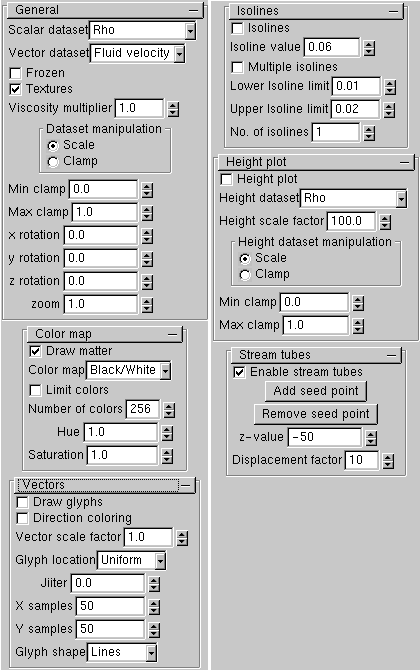
\includegraphics[width =0.5\textwidth]{content/pictures/menu.png}
            \caption{GLUI Menu}
            \label{fig:menu}
        \end{figure}